\documentclass[11pt]{article}

% ---------- page geometry and fonts ----------
\usepackage[a4paper,left=2.8cm,right=2.8cm,top=2.8cm,bottom=3.0cm]{geometry}
\usepackage[T1]{fontenc}
\usepackage[utf8]{inputenc}
\usepackage{mathptmx}
\usepackage{microtype}

% ---------- maths, tables, figures ----------
\usepackage{amsmath,amssymb,amsthm}
\usepackage{booktabs,threeparttable,graphicx}
\usepackage[font=small,labelfont=bf,skip=6pt]{caption}
\usepackage{setspace}
\usepackage{fancyhdr}
\usepackage[hidelinks,pdfusetitle]{hyperref}
\usepackage{natbib}
\bibpunct{(}{)}{;}{a}{}{,}

% ---------- spacing and layout ----------
\onehalfspacing
\setlength{\parindent}{1.5em}
\setlength{\parskip}{0pt}
\setlength{\abovedisplayskip}{10pt}
\setlength{\belowdisplayskip}{10pt}
\setlength{\abovedisplayshortskip}{6pt}
\setlength{\belowdisplayshortskip}{6pt}
\allowdisplaybreaks
\renewcommand{\arraystretch}{1.08}
\captionsetup[table]{position=top}
\captionsetup[figure]{position=bottom}

% ---------- headers ----------
\pagestyle{fancy}
\fancyhf{}
\fancyhead[L]{\small\itshape Central Bank Losses and Rate Advocacy}
\fancyhead[R]{\small\thepage}
\renewcommand{\headrulewidth}{0pt}
\fancypagestyle{plain}{\fancyhf{}\fancyfoot[C]{\small\thepage}\renewcommand{\headrulewidth}{0pt}}

% ---------- theorem environment ----------
\theoremstyle{plain}
\newtheorem{proposition}{Proposition}

% ---------- title ----------
\title{\bfseries Do Central Bank Losses Move Policymakers?\\[2pt]
\large Pre-Registered Evidence from the Eurosystem\thanks{Draft of 15 September 2026. The analysis plan and its four amendments were frozen with SHA-256 hashes before any rate-stance passage was read or coded, and the coded passages were frozen before being linked to institutions or dates. Measurement disclosure: passages were coded by a language model in a single pass, without an independent human validation sample; Section~\ref{sec:limits} discusses what this implies. The replication package contains the code, the hand-collected data, the frozen plan and codebook, and all coded passages.}}
\author{Philip Kroos}
\date{15 September 2026}

\begin{document}
\maketitle

\begin{abstract}\noindent\normalsize
Since 2022 most euro area national central banks (NCBs) have booked large losses on bond portfolios they bought under quantitative easing and must now fund at high policy rates. Whether such losses bend monetary policy is contested and, at the level of individual decision-makers, untested. We exploit a setting in which one policy is set by a committee whose members sit on 20 separate balance sheets: income from sovereign bonds bought since 2015 is neither risk- nor income-shared, so the carry loss per unit of capital key differs sharply across NCBs. We code 1{,}991 passages from speeches by NCB governors between 2016 and 2026 into a rate-stance scale and relate the stance to each NCB's non-pooled carry exposure, in a design registered in advance. We find no detectable effect: $0.03$ scale points per standard deviation of exposure, against a predicted positive coefficient (95\% CI $-0.33$ to $0.40$). Equivalence tests exclude effects larger than $0.34$ scale points, about forty per cent of the gap between the average German and the average Italian central banker, but cannot exclude smaller ones. The estimate is stable across twelve constructions of the exposure measure and eleven robustness checks. The event design around the first published net loss gives $-0.16$ and is not significant. The data are informative about why: governor and half-year fixed effects absorb 84\% of the variance of advocacy, leaving little room for any time-varying national condition. Stated policy preferences in the Governing Council look like a common cycle plus a stable individual type, with no detectable response to the finances of one's own institution.
\end{abstract}

\vspace{0.6em}
\noindent\textbf{Keywords:} central bank losses; quantitative easing; monetary policy committees; ECB Governing Council; text as data; pre-registration; null results.

\vspace{0.3em}
\noindent\textbf{JEL classification:} E52, E58, E42, D72, C93.

\clearpage

\section{Introduction}

Between 2022 and 2025 the Eurosystem lost money. The Deutsche Bundesbank published a record loss of more than EUR 19 billion for 2024 and a cumulative balance-sheet loss of EUR 27.8 billion by 2025; the Banque de France published EUR 7.7 billion for 2024; De Nederlandsche Bank, the National Bank of Belgium and N\'arodn\'a banka Slovenska had already published losses for 2022. The cause is mechanical. Under quantitative easing, national central banks (NCBs) bought long-dated sovereign bonds at very low fixed yields and funded them with reserves that are remunerated at the policy rate. When the policy rate rose from $-0.5\%$ to $4\%$, the funding cost rose with it and the asset yield did not.

Does this change how monetary policy is made? The question is old and unsettled. \citet{goncharov2023} show that central banks report small profits far more often than small losses, and that this pattern is stronger where governors face political pressure or can be reappointed. \citet{grodecka2025} find, over 350 years of Riksbank data, that exogenous falls in profits are followed by persistently higher inflation when the central bank is not automatically recapitalised. \citet{gebauer2024} compute that avoiding losses altogether would have required euro area policy rates of 1.7 to 2.5\% instead of the 2.5 to 3.6\% actually chosen, at a cost of up to half a percentage point of inflation per year. Central bankers themselves raise the question and answer it in the negative: one Governing Council member asks in a 2024 speech whether such losses impair the ability of central banks to apply their preferred policy rules or compromise their independence, and states that they do not.

What is missing is evidence at the level of the people who decide. Aggregate correlations between central bank capital and inflation cannot separate the finances of the institution from everything else that moves with them, and a single central bank over time has no control group. This paper supplies the missing test.

\paragraph{Setting.} The euro area offers an unusual laboratory: one monetary policy, one committee, and twenty separate balance sheets. Government and agency bonds bought since 2015 are neither risk-shared nor income-shared \citep{arrata2026}. Each NCB holds the bonds of its own jurisdiction and pays the reference rate on the pooled funding behind them. Everything else is pooled and identical per unit of capital key. The NCB-specific component of income is therefore the carry on its own portfolio, and it differs sharply: the average purchase yield of own holdings at the end of 2021 ranged from $-0.41\%$ in Luxembourg and $-0.36\%$ in Germany to $1.25\%$ in Portugal and $1.32\%$ in Italy. Governors of these institutions sit in the same room and vote on the same policy.

\paragraph{What we do.} We build a governor-level measure of stated rate preferences. From the BIS full-text archive we take every speech by a head of a euro area NCB between January 2016 and June 2026, split the texts into five-sentence passages, mask speaker names, institutions, roles, countries and cities, and keep the 1{,}991 passages that match a rate-stance filter. Each passage is coded as favouring lower rates ($-1$), neutral ($0$) or favouring higher rates ($+1$), blind to institution and date. We construct each NCB's non-pooled carry from public ECB data and validate it against reported net interest income. We then estimate the relation between exposure and stance with governor and half-year fixed effects, with inference by permutation of NCB exposure paths.

The design, the outcome, the controls, the inference and the interpretation rules were fixed in a pre-analysis plan and four dated amendments, each frozen with a hash, before any stance passage was read. The plan itself replaced our first intended outcome -- advocacy on reserve remuneration -- after a pre-specified count rule showed it was too rare in speeches to be measurable. The amendments were then triggered by an ex-ante power calculation, by a bad-control concern about contemporaneous macro controls, by a simulation showing that our planned inference had a rejection rate of 9\% under the null, and by a diagnostic showing that the identifying variation is concentrated in two NCBs.

\paragraph{Result.} Exposure does not move advocacy. The point estimate is $+0.034$ scale points per standard deviation of exposure, with a standard error of $0.187$; the permutation $p$-value is $0.81$ from 999 permutations. The sign is the one the model predicts, and the magnitude is negligible: an NCB one standard deviation deeper in loss territory has a governor whose advocacy is three hundredths of a scale point more dovish. The estimate is between $0.033$ and $0.046$ across all twelve pre-specified constructions of the exposure measure, between $-0.06$ and $+0.11$ across eleven robustness checks, and between $-0.13$ and $+0.11$ when each NCB in turn is dropped. Leads of exposure are jointly indistinguishable from zero. The event design around the first published net loss gives $-0.16$ scale points with $p=0.51$, in the hypothesised direction but not distinguishable from placebo event dates, and known ex ante to be underpowered.

We are careful about what this rules out. The confidence interval runs from $-0.33$ to $+0.40$ scale points. The design was built to detect $0.27$ points with 80\% probability and it does not detect anything of that size; it cannot exclude smaller effects.

\paragraph{Why the null is informative.} The same data show where advocacy does come from. Governor fixed effects alone explain 49\% of the weighted variance of the stance measure, half-year fixed effects alone 42\%, and the two together 84\%. What remains for any time-varying national condition -- losses, spreads, debt -- is 16\% of the variance, and exposure explains none of it. Pre-period debt interacted with the policy rate, the channel documented by \citet{heinemann2026}, is equally flat once exposure is included. National differences in advocacy are large (Germany $+0.51$, Italy $-0.36$ on a $-1$ to $+1$ scale) but they are persistent, not cyclical: they live in the fixed effects.

\paragraph{Related literature.}
The paper speaks to four strands.

The first asks whether central bank finances influence central bank behaviour. \citet{goncharov2023} document a discontinuity in the distribution of reported central bank profits at zero, show that it is stronger where governors face political pressure or are eligible for reappointment, and relate it to policy rules and inflation; their identification is cross-institutional and predates the loss episode. \citet{grodecka2025} use 350 years of Riksbank data and narrative identification to show that exogenous falls in profits are followed by higher inflation when the institution is not automatically recapitalised. \citet{gebauer2024} quantify what avoiding losses would have cost in inflation terms for the euro area. \citet{cecchetti2024} set out the fiscal arithmetic and stress how accounting conventions and indemnification arrangements determine what is visible. A separate policy literature argues the opposite side, finding no association between central bank capital and subsequent inflation. Our contribution is to move the question to the level of the individual decision-maker, using variation that is predetermined by purchases made before the episode.

The second strand concerns how the stated preferences of policymakers are measured. \citet{bennani2017} code 1{,}618 speeches by Governing Council members with a dictionary approach and find a home bias in expressed hawkishness. \citet{heinemann2026} code 4{,}680 speeches with a language model and relate members' stated objectives to public debt at home, describing their own approach as forensic rather than causal. \citet{hansen2018} exploit FOMC transcripts to study how transparency changes deliberation. We adopt the passage-level unit and the model-assisted coding of this literature, and add masking, blind coding, and a pre-registered design; we also extend the window through the loss episode itself, which earlier corpora do not cover.

The third is the political economy of monetary committees. \citet{moschella2020} show that dissent from the line taken by the ECB President tracks the ideology of the speaker's home government. Recent work links politically motivated governor appointments to more dovish expectations and to higher inflation \citep{imf2026governors}, and \citet{bartels2026} show that more independent central banks took more financial risk at the effective lower bound -- a result that matters here because it suggests exposure could proxy for institutional traits. Our governor fixed effects absorb stable traits of this kind, and the capital key allocation of purchases limits how much discretion NCBs had over the exposure in the first place.

The fourth is the design literature we borrow from: heterogeneity-robust event-study estimation \citep{borusyak2024,callaway2021}, and permutation and bootstrap inference for settings with few effective clusters. Our contribution here is practical rather than methodological: we document, in simulations calibrated to our own data, that two natural choices of test statistic reject a true null in 17\% and 9\% of cases, and that a jackknife-studentised statistic restores nominal size.

\paragraph{Contribution.}
Relative to \citet{goncharov2023} we move from a cross-section of institutions to individuals inside one committee facing one policy, with exposure that is predetermined by purchases made before the loss episode. Relative to \citet{grodecka2025} we have 17 institutions rather than one, and an outcome measured at the level of the decision-maker. Relative to \citet{heinemann2026} we add a different and more directly financial channel, a design registered in advance, and the 2024 to 2026 period in which the losses actually materialised. The paper also contributes two reusable public-data objects: a hand-collected record of NCB results, provisions and distributions with a source for every entry, and a construction of non-pooled carry exposure from published ECB purchase data that reproduces the reported ranking of net interest income across the four largest NCBs. Finally, the sequence of pre-registered amendments is itself informative for work of this kind: a count rule killed our sharpest outcome before we could be tempted by it, a power calculation demoted our most intuitive design, and a size simulation replaced our planned inference.

Section~\ref{sec:inst} describes how losses are allocated inside the Eurosystem, Section~\ref{sec:model} sets out what a loss-averse policymaker would do, Section~\ref{sec:data} the measurement, Section~\ref{sec:strategy} the design, Section~\ref{sec:results} the results, and Section~\ref{sec:limits} what we can and cannot conclude.

\section{Institutional background: how losses land on national central banks}\label{sec:inst}

\paragraph{How monetary income is pooled.}
Article~32 of the Statute requires that the income accruing to NCBs from the performance of monetary policy functions be pooled and redistributed in proportion to paid-up shares in ECB capital. The implementing decision identifies the liability base -- essentially banknotes in circulation and reserves held by counterparties -- and a set of earmarkable assets held against it. Where an NCB's earmarkable assets fall short of its liability base, the shortfall is a pooled net asset on which it receives the reference rate; where they exceed it, it pays the reference rate on the excess. The reference rate was the rate on the main refinancing operations until the end of 2024 and has been the deposit facility rate since 1 January 2025 \citep{arrata2026}. The consequence is that the cost of remunerating reserves is shared: per unit of capital key it is identical across NCBs, and in an estimating equation with time fixed effects it is absorbed entirely.

\paragraph{What is not pooled.}
Sovereign and agency bonds purchased since 2015 under the public sector purchase programme and the pandemic emergency purchase programme are the exception. Each NCB buys the bonds of its own jurisdiction, the great majority of the associated risk is excluded from risk-sharing, and the income is not pooled \citep{arrata2026}. An NCB that bought at low yields therefore earns little on those bonds while paying the reference rate on the pooled funding behind them, and the resulting carry is its own. The NCB-specific component of net income is therefore the carry on its own portfolio,
\begin{equation}\label{eq:carry}
\text{carry}_{n,t} \;=\; S_{n,t}\,\bigl(s_{n,t} - r^{\text{ref}}_t\bigr),
\end{equation}
where $S_{n,t}$ denotes NCB $n$'s own holdings, $s_{n,t}$ their average purchase yield and $r^{\text{ref}}_t$ the reference rate. Everything else in the profit and loss account that arises from monetary policy is common per unit of capital key.

This is the variation the paper uses. Its size is not trivial: one governor told the audience at his institution's annual accounts press conference that with an interest rate exposure of around EUR 300 billion, a one percentage point increase in policy rates costs roughly EUR 3 billion a year, and that the balance sheet had been effectively free of interest rate risk when monetary policy was implemented through short-term operations alone.

\paragraph{Accounting conventions matter for which instrument hurts.}
Monetary policy securities are carried at amortised cost subject to an impairment test \citep{gebauer2024}. Unrealised price losses on bonds bought at low yields therefore do not pass through the profit and loss account. A loss is booked when the carry is negative, which happens automatically once the policy rate exceeds the portfolio yield, and it would be booked at once if bonds were sold. Passive run-off, by contrast, removes the exposure without realising anything. A policymaker who cared about the published result would therefore have a clear preference ordering over instruments -- against sales, in favour of run-off, and above all in favour of a lower remuneration of reserves -- which is what motivates the model in Section~\ref{sec:model}.

\paragraph{From economic loss to published loss: buffers.}
Whether a negative carry becomes a published loss depends on provisions built in earlier years, and these differ. Table~\ref{tab:losses} summarises our hand-collected record. Three NCBs published net losses already for 2022: De Nederlandsche Bank (EUR 460 million), the National Bank of Belgium (EUR 580 million, its first loss in roughly seventy years) and N\'arodn\'a banka Slovenska. The Oesterreichische Nationalbank followed for 2023 with EUR 2.2 billion, and reported negative equity for the first time for 2024. The Bundesbank reported a zero result for 2023 only because it released provisions, then a record loss of more than EUR 19 billion for 2024 and EUR 8.6 billion for 2025, bringing the loss carried forward to EUR 27.8 billion; 2025 was its sixth consecutive year without a transfer to the federal budget. The Banque de France reported a pre-tax loss of EUR 17.4 billion for 2024, released EUR 10.1 billion of its fund for general risks and published EUR 7.7 billion, before returning to profit in 2025.

Others absorbed comparable pre-provision losses without publishing one. The Banco de Espa\~na covered an operating loss of EUR 7.5 billion for 2024 in full and published a zero result. Suomen Pankki covered EUR 1.0 billion for 2024 by exhausting its general provision and drawing EUR 241 million from its provision against real value loss. The Banco de Portugal turned a pre-provision loss of EUR 1.1 billion into a net profit of EUR 1.5 million through deferred taxes. The Central Bank of Ireland covered losses of EUR 132 million and EUR 795 million with its financial risk reserve and transferred nothing to the Exchequer. The Banca d'Italia turned a gross loss of EUR 7.3 billion for 2024 into a net profit of EUR 844 million, of which EUR 644 million went to the Treasury and EUR 200 million to its private participants. The Bank of Greece is the only NCB in our record with no pre-provision loss at all, which is consistent with the high yields on the domestic bonds it holds.

This heterogeneity is useful twice over. It supplies the staggered timing of our secondary design, and it separates the economic burden from its visibility: Finland and the Netherlands bear similar carry per unit of capital key, and only one of them published a loss.

\begin{table}[t]\centering\small
\begin{threeparttable}
\caption{First published losses by national central bank}\label{tab:losses}
\begin{tabular}{lcccl}
\toprule
NCB & Pre-provision loss & Net loss & Treated from & Note \\
\midrule
NL, BE, SK & FY2022 & FY2022 & 2023H2 & BE: first loss in $\approx$70 years \\
AT & FY2023 & FY2023 & 2024H2 & negative equity from FY2024 \\
DE & FY2023 & FY2024 & 2025H2 & loss carried forward EUR 27.8bn \\
FR & FY2023 & FY2024 & 2025H2 & profit again in FY2025 \\
ES, IT, FI, PT, IE & FY2023 & none & never & covered by provisions \\
LU & n.a. & none & never & balanced results reported \\
GR & none & none & never & high-yielding own portfolio \\
\bottomrule
\end{tabular}
\begin{tablenotes}\footnotesize
\item \textit{Notes:} Hand-collected from NCB annual accounts, press releases, audit reports and press coverage of the accounts, with one source per NCB-year recorded in the replication package. A net loss reduces equity or is carried forward after provisions have been used. Technical losses arising from deferred taxes (Portugal, FY2025) are excluded. ``Treated from'' is the first half-year beginning after publication; the half-year of publication is dropped in estimation, and where the publication date is not documented it is set to 31 March of the following year. FY2025 results for IE, GR and LU are not yet documented; a net loss there would affect 2026H1 only. LT, EE, LV, HR, CY, MT and SI are excluded from the event design until their status is documented, and enter the exposure design only.
\end{tablenotes}
\end{threeparttable}
\end{table}

\paragraph{What losses do and do not imply.}
No euro area NCB is obliged to be recapitalised, and none has been. Losses are carried forward against future profits; national statutes differ in whether and how reserves may be drawn on. The immediate fiscal consequence is the absence of a transfer to the treasury rather than a payment from it. Two NCBs, the National Bank of Belgium and the Bank of Greece, are listed companies with private shareholders, which adds an audience: the Belgian share price fell by more than a quarter on the day the first loss was announced, and the Council of Regency later changed the reserve and dividend policy to prioritise rebuilding reserves. \citet{cecchetti2024} put the maximum annual loss at 0.3 to 1.5\% of GDP for the Federal Reserve, the Eurosystem and the Bank of England, against 17\% for the Swiss National Bank, and stress that accounting rules and indemnification arrangements determine how much of this is visible.

\paragraph{The instrument the accounting points to.}
The cheapest way to reduce the loss is to pay less on reserves. Minimum reserve requirements have stood at 1\% of the relevant liability base since 2012, and their remuneration was set to zero with effect from 20 September 2023; the average reserve requirement was EUR 169.6 billion in the maintenance period ending in February 2026. Proposals to raise the ratio substantially, and thereby to enlarge the unremunerated share, have been made repeatedly in the policy debate, and press reporting in 2026 indicated that a doubling to 2\% was under consideration in part because it would reduce NCB losses. This is the instrument on which a policymaker who weighted the published result would reveal herself most cleanly, and Section~\ref{sec:data} explains why we could not measure advocacy on it.

\paragraph{Who decides.}
The Governing Council consists of the six members of the Executive Board and the governors of the NCBs -- twenty during our sample, twenty-one after Bulgaria adopted the euro in January 2026. Individual votes are not published and no minutes attribute positions to named members, so the observable record of individual preferences is what members say in public. They say a great deal: the BIS archive contains 1{,}347 speeches by euro area NCB heads in our window. Executive Board members serve non-renewable eight-year terms and have no national treasury as a residual claimant on their institution's profit; governors' terms are set nationally, and several of those in office during the loss episode were previously ministers in their own governments. Between 2024 and 2026 at least seven NCBs changed governor, among them France, Spain, Austria, Slovenia, the Netherlands and Portugal. The design accounts for turnover with governor fixed effects and with a robustness check that drops successors appointed after exposure had risen.

\section{A model of advocacy with heterogeneous balance sheets}\label{sec:model}

The model has one purpose: to say which instrument a policymaker who cares about her own institution's result would push, and in which direction, so that the empirical work is not a fishing exercise. It is deliberately small.

\paragraph{Setup.}
Governor $i$ states preferred settings for three instruments: the policy rate $r$, the share $q\in[0,1]$ of reserves that is not remunerated, and active sales $a$ of her own sovereign portfolio. She minimises
\begin{equation}\label{eq:loss}
L_i \;=\; \underbrace{\tfrac12\,(g_i - \kappa r - \eta a)^2}_{\text{stabilisation}} \;+\; \tfrac12 \phi r^2 + \tfrac12 \zeta a^2 + \tfrac12 \chi q^2 \;-\; \omega_i\,\Pi_i(r,q,a),
\end{equation}
where $g_i$ is perceived inflation pressure and $\kappa,\eta>0$ measure how strongly the rate and sales tighten conditions. The three quadratic terms are the costs of using each instrument: $\phi$ captures the output and financial-stability cost of the rate itself, without which the rate would be a free instrument and sales would never be used; $\zeta$ the disruption cost of selling into the market; $\chi$ the implementation cost of an unremunerated reserve requirement, which acts as a tax on banks.

The NCB result per unit of capital key is
\begin{equation}\label{eq:pnl}
\Pi_i \;=\; S s_i \;-\; (1-q)\,D\,r \;+\; B\,r \;-\; a\,\delta\,(r - s_i),
\end{equation}
with $S$ the own sovereign portfolio at purchase yield $s_i$, $D$ reserves and $B$ banknotes per unit of key, and $\delta$ the duration realised on sale. Reserves and banknotes are pooled and therefore common across NCBs per unit of key; $s_i$ and $\delta$ are not. The final term is the loss crystallised by selling bonds bought at $s_i$ when the market rate is $r$.

\paragraph{The weight on own profit.}
The parameter of interest is
\begin{equation}\label{eq:omega}
\omega_i \;=\; \psi_i\,\bigl(1 + \ell\cdot\mathbf{1}\{\Pi_i + \text{buffer}_i < 0\}\bigr),
\end{equation}
where $\psi_i \geq 0$ is the weight the governor places on her institution's result in normal times -- shaped by fiscal backing, by statute, and by political pressure -- and $\ell \geq 0$ is additional weight that switches on when the published result turns negative. The indicator is what makes buffers matter: two NCBs with the same economic carry differ in $\omega$ if one can absorb the loss with provisions and the other cannot. Equation~\eqref{eq:omega} is the formal counterpart of the institutional discussion in Section~\ref{sec:inst} and of the pattern in Table~\ref{tab:losses}.

\paragraph{Comparative statics.}
Let $x^* = (r^*, q^*, a^*)$ solve the first-order conditions of \eqref{eq:loss} at an interior optimum satisfying the second-order conditions. Applying the implicit function theorem to the system gives the results below; proofs and the numerical verification are in Appendix~\ref{app:model}.

\begin{proposition}[Rate advocacy]\label{prop:rate}
At an interior optimum satisfying the second-order condition, $\partial r^*/\partial \omega_i < 0$ if and only if
\begin{equation}\label{eq:cond}
(1-q^*)D - B + a^*\delta \;>\; q^* D \;+\; \frac{\delta\,(r^*-s)\,(\omega\delta + \kappa\eta)}{\eta^2+\zeta}.
\end{equation}
If the sales channel is inactive ($\delta = 0$ or $a^*=0$), the condition reduces to $D\,(1-2q^*) > B$.
\end{proposition}

The proposition is stated as an equivalence rather than as an unconditional prediction, because the sign is not determined by the second-order condition alone: raising $\omega$ makes the governor want a lower rate through the reserve-remuneration term but also want more sales, which pushes the rate back up. The left-hand side of \eqref{eq:cond} is the sensitivity of the published result to the policy rate; the right-hand side collects the two offsetting effects.

The special case of the condition is satisfied by a wide margin in our setting. In the special case it requires reserves, net of twice the unremunerated share, to exceed banknotes in circulation. Excess reserves in the euro area have exceeded banknotes continuously since 2015, and the unremunerated share has been at most one per cent of the reserve base, so $D(1-2q^*)$ exceeds $B$ by a wide margin. The general condition adds a term in $\delta(r^*-s)$ that is small whenever \emph{advocated} sales are small. We cannot observe $a_i^*$: no NCB sold sovereign holdings outright during the sample, but realised policy is a committee outcome and need not equal any member's preferred setting. We therefore rely on the special case, which is empirically compelling, and on the numerical check reported in Appendix~\ref{app:model}, which finds the condition satisfied in every admissible parameter draw with $\Lambda>0$. Within the empirically relevant region, therefore, a governor who weights her own result advocates a lower policy rate, and this is the prediction we take to the data.

\begin{proposition}[Revealed profit monotonicity]\label{prop:pnl}
For any cost function satisfying the second-order conditions, the result implied by the advocated instrument mix, $\Pi_i(x^*(\omega_i))$, is weakly increasing in $\omega_i$.
\end{proposition}

Proposition~\ref{prop:pnl} is weaker but more robust than Proposition~\ref{prop:rate}: it does not depend on which instrument does the work. It motivates the pooled profit-implied index we report as a secondary outcome.

\begin{proposition}[Pooled instruments require a kink]\label{prop:kink}
Let $q_i^\dagger(r_t)$ denote governor $i$'s preferred unremunerated share evaluated at the prevailing policy rate $r_t$, rather than at her own preferred rate. Then $q_i^\dagger(r_t) = \omega_i D r_t/\chi$, so that at a given date any cross-sectional difference in $q^\dagger$ arises only through $\omega_i$ (or through $\chi_i$), and not through the preference shifter $g_i$.
\end{proposition}

The conditioning matters. Evaluated at each governor's own preferred rate, $q_i^* = \omega_i D r_i^*/\chi$ would differ across governors merely because $r_i^*$ differs with $g_i$, and the instrument would no longer be clean. Evaluated at the rate that actually prevails -- which is the relevant object, since reserve remuneration is a decision taken at a given policy rate -- the preference shifter drops out. This is the sharpest implication of the model and the reason our original design targeted reserve remuneration. Because the marginal saving $Dr_t$ is common across NCBs per unit of capital key, with common $\psi$ and common $\chi$ linear concern for profit alone cannot generate cross-sectional disagreement about $q^\dagger$; the loss indicator in \eqref{eq:omega} generates an additional time-varying wedge around zero. Advocacy on reserve remuneration would therefore have identified loss aversion among central bankers separately from any preference shifter. Section~\ref{sec:data} explains why the corpus cannot support that test.

\paragraph{Two predictions that do not survive.}
Two intuitive implications fail verification and we do not use them. The first is that loss-averse governors oppose asset sales, because sales crystallise losses. It holds in only 65 of 266 admissible parameter draws: a governor who cuts the costly policy rate substitutes into sales, and when the loss per euro sold, $\delta(r-s_i)$, is small relative to the rate exposure, the substitution dominates. The second is that longer portfolio duration reduces advocated sales; it holds in 251 of 266 draws, because duration raises both the loss per sale and the rate exposure. We report both failures because they discipline the empirical work: without the check we would have tested a sign pattern on asset sales that the model does not in fact imply.

\paragraph{From individual advocacy to committee outcomes.}
The Governing Council decides by consensus, with a vote as the fallback, so the mapping from stated preferences to outcomes is an aggregation problem. If the decision is the median of the members' preferred settings, the effect of losses on policy is $\partial r^{\text{med}}/\partial \omega$ evaluated at the median member, which is zero unless the median member's own institution is exposed. Twenty-one voting rights are exercised at any meeting, six of them held permanently by Executive Board members who have no national institution behind them, and the remaining fifteen rotating among the governors. Any individual incentive is therefore diluted substantially. This matters for interpretation: a null on individual advocacy is stronger evidence against the mechanism than a null on realised policy would be, because aggregation can only attenuate. It also explains why the test is worth running at the level of the individual at all.

\section{Data and measurement}\label{sec:data}

\paragraph{Speeches.}
Our corpus is the full-text extract of central bankers' speeches compiled by the Bank for International Settlements, which covers speeches, lectures, interviews and parliamentary statements that central banks submit to it. Between January 2016 and June 2026 it contains 8{,}672 speeches worldwide, of which 1{,}347 were given by heads of euro area NCBs and 1{,}019 by members of the ECB's Executive Board.

The archive records no institution field, so affiliation has to be recovered from the description line, which follows a stable pattern: type of remarks, speaker name, role, institution, venue, place and date. We remove the speaker's name, cut the string at the first venue marker, and match institution aliases only inside the remaining affiliation segment, so that a speech hosted by another central bank is not misattributed. Roles containing deputy, vice, member, director, chief, adviser or head of are classified as non-heads. The parser passes twelve unit tests written against real description strings, including joint speeches by two officials and speeches by non-euro-area speakers at euro area events, and its output is consistent with the archive's own author field in 99.7\% of cases.

Texts are split into five-sentence passages, following \citet{heinemann2026}, with a rule-based splitter that protects abbreviations, initials and decimals in six languages. This yields 28{,}558 passages by NCB heads and 24{,}157 by Board members.

\paragraph{What the corpus can and cannot measure.}
Our pre-registered first outcome was advocacy on the remuneration of reserves, the instrument identified by Proposition~\ref{prop:kink}. A count rule fixed in advance required at least one relevant passage per NCB half-year and relevant passages from at least twelve NCBs. The corpus delivers 0.38 passages per cell and nine NCBs, and this is an upper bound, since roughly half the keyword matches are descriptive uses of ``excess liquidity''. Following the rule, we abandoned that outcome before reading or coding any position. Rate advocacy is an order of magnitude more frequent: 6.8 keyword-matched passages per NCB half-year from eighteen NCBs, balanced between NCBs that later published net losses (571 passages) and those that did not (600).

The scarcity is not an artefact of the filter. A moderate expansion of the keyword list raises matched passages in the 2022--2026 window from 1{,}218 to 1{,}634 but changes almost nothing for the small NCBs, because the binding constraint is the supply of speeches: Eesti Pank and N\'arodn\'a banka Slovenska each have two speeches in the archive over the whole window.

\paragraph{Classification.}
We classify the 1{,}991 passages by NCB heads that match the rate-stance filter. Speaker names, institution names and aliases, role phrases, country names, demonyms and 21 capitals and major cities are replaced by placeholders before coding; an automated scan finds residual country cues in three of 400 audited passages. Each passage is coded on three dimensions: whether it states a view on the direction, level or pace of policy rates or on the overall stance; if so, whether that view favours lower rates ($-1$), is neutral ($0$), or favours higher rates ($+1$); and whether it evaluates only past decisions. The codebook, including the decision rules for the recurring borderline cases discussed in Section~\ref{sec:measure}, was frozen before coding and is reproduced in Appendix~\ref{app:codebook}.

Coding was performed in a single pass by a language model working from the frozen codebook, with passages presented in random order under opaque identifiers, and was completed and hash-frozen before any passage was linked to an institution or a date. The estimation code refuses to run against results whose hash does not match. In the event, the validation sample was not coded by humans: all passages were coded in a single model pass. No agreement statistics and no estimate of filter recall are therefore available, and Section~\ref{sec:limits} treats this as the paper's main measurement limitation.

\paragraph{Exposure: construction.}
We build the carry of equation~\eqref{eq:carry} for 19 NCBs from public ECB data. Holdings $S_{n,t}$ are cumulative monthly net purchases by jurisdiction under the PSPP and the PEPP, as published by the ECB; our parser reproduces the published figures exactly (for example EUR 435{,}323 million for Germany under the PSPP at end-August 2026). We scale them by the NCB share of jurisdiction holdings, $8/9$, since ten per cent of purchases were made by the ECB itself. The purchase yield $s_{n,t}$ is built recursively: each month's gross purchases enter at the national yield for the portfolio's weighted average maturity, and the stock yield is the purchase-weighted average of what came before and what is added. National yields are the ten-year series from the ECB's convergence statistics, shifted to the relevant maturity using the slope of the AAA euro area curve, because longer maturity series are not available for every country. The reference rate is the monthly average main refinancing rate until December 2024 and the deposit facility rate from January 2025. Carry is divided by the Eurosystem capital key, demeaned across NCBs within each half-year and standardised.

\paragraph{Exposure: a worked example.}
In December 2023 the Bundesbank's own PSPP and PEPP holdings were EUR 895 billion at an average purchase yield of $-0.27\%$, against a reference rate of $4.5\%$. The implied annual carry is $895 \times (-0.0027 - 0.045) = -\text{EUR }42.7$ billion, or EUR 1.60 billion per percentage point of capital key. The corresponding figures are EUR 1.53 billion for France, EUR 1.32 billion for Spain and EUR 1.19 billion for Italy, whose portfolio yielded $1.44\%$. Demeaning within the half-year leaves Germany EUR 0.59 billion per key point below the Eurosystem average and Italy EUR 0.18 billion below it: the ordering the estimator uses.

\paragraph{Exposure: validation.}
The only published counterpart is net interest income after reallocation, which \citet{arrata2026} report for the four largest NCBs in 2023 and 2024. Per percentage point of capital key those figures are EUR $-0.71$ and $-0.69$ billion for Germany, $-0.74$ and $-0.80$ for France, $-0.48$ and $-0.54$ for Spain, and $-0.37$ and $-0.38$ for Italy. Our measure reproduces the level ordering of Italy below Spain and both below the core, with a rank correlation of $0.79$; it does not reproduce the reversal by which France loses more per key point than Germany. Two things explain the gap. Reported net interest income includes non-pooled items beyond the sovereign portfolio, in particular each NCB's own funds and foreign reserve portfolios, and our construction abstracts from differences in the timing of purchases within a month. We treat this as a limitation of the measure rather than a validation failure, and it is the reason the pre-analysis plan designated the published-loss design, rather than the carry measure, as the fallback should the two disagree. Across the twelve pre-specified constructions the correlation with the baseline measure after 2021 is at least $0.98$ and the rank correlation with reported income lies between $0.74$ and $0.81$.

\paragraph{Controls.}
The pre-analysis plan specified three controls: national HICP inflation and the 2019--2021 averages of the ten-year spread to Germany and of the general government debt ratio, each interacted with the deposit facility rate. The two pre-period controls enter all main specifications. National HICP does not: it could not be retrieved before estimation and its omission is recorded as a deviation. Since the plan is frozen we do not add it silently to the main specification. We note that the specification without any controls (R4) is \emph{not} a bound on the influence of an omitted confounder: if national inflation correlates with both exposure and advocacy, dropping the remaining controls says nothing about what including inflation would do. Adding national HICP as a clearly labelled post-registered robustness check is the appropriate remedy. We were unable to assemble the series for the full country panel from the sources available to us, and record this as an open item in Appendix~\ref{app:prereg} rather than substituting a weaker proxy. The debt ratio absorbs the channel documented by \citet{heinemann2026}. Debt ratios are taken from Eurostat's October 2022 notification of deficit and debt data. Dropping the controls entirely changes the estimate from $0.034$ to $0.016$ (Table~\ref{tab:main}, R4). This bounds the influence of the controls we do include. It says nothing about the omitted inflation control, which remains an open item.


\section{The stance measure}\label{sec:measure}

Before using the measure we document what it contains. All the facts in this section were invisible at the coding stage: institutions, roles, countries, cities and dates were masked, and passages were presented in random order.

\paragraph{Coverage.}
Table~\ref{tab:desc} reports coverage by NCB. Of the 1{,}991 coded passages, 1{,}248 state a view on the policy rate and enter the panel, spread over 168 governor half-years, 31 governors and 17 NCBs. Coverage is very uneven. Germany contributes 306 coded passages and France 209, while Slovakia contributes two and Slovenia four. The reason is the supply of speeches, not the filter: Eesti Pank and N\'arodn\'a banka Slovenska each have two speeches in the BIS archive over the whole eleven-year window, against 186 for the Bundesbank. Weighting by passage counts, as our estimator does, means that the large NCBs carry the estimate; the leave-one-out exhibit in Section~\ref{sec:results} shows what happens when each is removed in turn.

\begin{table}[t]\centering\small
\begin{threeparttable}
\caption{Coded passages and average stance by national central bank}\label{tab:desc}
\begin{tabular}{lrrrrr}
\toprule
NCB & Governor half-years & Coded passages & Governors & Mean stance & Mean exposure \\
\midrule
Germany & 21 & 306 & 2 & $0.51$ & $-1.17$ \\
France & 21 & 209 & 2 & $-0.22$ & $-0.60$ \\
Italy & 20 & 171 & 2 & $-0.36$ & $0.63$ \\
Spain & 17 & 154 & 3 & $0.02$ & $0.46$ \\
Finland & 17 & 116 & 2 & $-0.18$ & $-0.74$ \\
Netherlands & 15 & 104 & 2 & $0.12$ & $-0.88$ \\
Ireland & 14 & 49 & 2 & $0.18$ & $-0.17$ \\
Greece & 17 & 46 & 1 & $-0.22$ & $0.98$ \\
Belgium & 4 & 39 & 2 & $0.31$ & $-0.74$ \\
Malta & 4 & 18 & 2 & $0.22$ & $0.78$ \\
Portugal & 2 & 7 & 1 & $-0.71$ & $1.25$ \\
Cyprus & 3 & 7 & 2 & $0.00$ & $0.54$ \\
Estonia & 2 & 6 & 1 & $0.67$ & $2.23$ \\
Austria & 3 & 5 & 1 & $0.40$ & $-1.38$ \\
Lithuania & 3 & 5 & 2 & $0.40$ & $-0.34$ \\
Slovenia & 3 & 4 & 2 & $0.75$ & $-0.42$ \\
Slovakia & 2 & 2 & 2 & $0.50$ & $-0.02$ \\
\midrule
Total & 168 & 1{,}248 & 31 & $0.05$ & \\
\bottomrule
\end{tabular}
\begin{tablenotes}\footnotesize
\item \textit{Notes:} Passages by heads of euro area NCBs in the BIS speech archive, 2016H1--2026H1, that match the rate-stance keyword filter and were coded as stating a view on the policy rate. Stance is the passage-weighted mean on a $-1$ (favours lower rates) to $+1$ (favours higher rates) scale. Exposure is the mean standardised non-pooled carry per percentage point of capital key; more negative values mean larger losses. Greece has no PSPP holdings and enters the exposure measure from 2020. Luxembourg has no coded passage in the window and does not appear.
\end{tablenotes}
\end{threeparttable}
\end{table}

\paragraph{The measure tracks policy, and leads it.}
The passage-weighted mean stance moves from $-0.25$ over 2016--2021 to $+0.40$ over 2022--2023 and back to $-0.08$ over 2024--2026 (Figure~\ref{fig:stance}, panel A). Its correlation with the level of the deposit facility rate is $0.45$ and with the contemporaneous change in that rate $0.58$. The correlation with the change in the following half-year is $0.62$: advocacy moves before policy does, which is what one would expect of a measure of stated preferences rather than of policy outcomes, and which no step of the coding could have engineered.

\paragraph{The measure reproduces the known ordering of the committee.}
Germany is the most hawkish of the well-covered NCBs at $+0.51$ and Italy the most dovish at $-0.36$, with France, Greece and Finland below zero and the Netherlands, Ireland and Belgium above. Restricting to NCBs with at least twenty coded passages, the standard deviation of average stance across NCBs is $0.30$ and across governors $0.51$. These differences are large relative to anything time-varying in the data, and they are the reason the paper leans on fixed effects.

\paragraph{The measure contains genuine disagreement, not committee boilerplate.}
If speeches merely restated Governing Council decisions, the cross-section would be flat and the design would have nothing to work with. It is not. Coded passages include explicit dissent -- one speaker recounts disagreeing with the July 2021 forward guidance and dissenting repeatedly thereafter; another states that he is more sceptical than many colleagues, particularly on government bond purchases; a third reports having called for a hike of at least 200 basis points to bring real rates to zero. Passages of this kind are why individual-level variation exists at all.

\paragraph{Borderline cases and how they were handled.}
Roughly one passage in ten required a judgement that the codebook resolves but that a reasonable coder could resolve differently. The most frequent is the formula that rates ``have reached levels that, maintained for a sufficiently long duration, will make a substantial contribution'': it asks for neither an increase nor a decrease and is coded neutral throughout. The second is the combination of a defence of past tightening with the observation that much of its effect is still in the pipeline; without an explicit direction this too is neutral. The third is the pipeline argument on its own -- ``most of the economic impact of rate hikes is yet to be felt, suggesting a degree of prudence'' -- which is coded as favouring lower rates, because the operative recommendation is caution against further tightening. Coding these three families differently would move the measure; Section~\ref{sec:limits} explains why we cannot bound by how much.

\section{Empirical strategy}\label{sec:strategy}

The specifications in this section were fixed in a pre-analysis plan and four dated amendments before any rate-stance passage was read, coded or linked to its institution. Every amendment was triggered by a pre-specified step that used only counts, treatment data or simulations, never outcomes. All documents are hash-frozen in the replication package.

\paragraph{Unit and outcome.}
The unit of observation is a governor in a half-year between 2016H1 and 2026H1. The outcome $y_{g,t}$ is the mean coded position ($-1$, $0$, $+1$) across all rate-stance passages of governor $g$ in half-year $t$. Cells without a rate-stance passage are dropped. Estimation weights are the number of passages in a cell.

\paragraph{Primary design: exposure.}
Our primary specification relates rate advocacy to the NCB-specific carry in equation~\eqref{eq:carry},
\begin{equation}\label{eq:dose}
y_{g,t} = \alpha_g + \gamma_t + \beta\, E_{n(g),t} + X_{n(g),t}'\delta + \varepsilon_{g,t},
\end{equation}
where $E_{n,t}$ is the non-pooled carry per percentage point of capital key of governor $g$'s central bank $n(g)$, demeaned across NCBs within each half-year and standardised. Governor fixed effects $\alpha_g$ absorb time-invariant preferences, including national traditions of hawkishness. Half-year fixed effects $\gamma_t$ absorb the common policy cycle and all pooled components of NCB income. The controls $X_{n,t}$ are the 2019 to 2021 averages of the ten-year spread to Germany and of the general government debt ratio, each interacted with the deposit facility rate. We use pre-period levels because contemporaneous spreads and debt respond to the same policy decisions. National HICP inflation was specified in the plan but could not be retrieved before estimation; it is absent from all specifications reported here, and Appendix~\ref{app:prereg} records the deviation. Note the sign convention: $E$ is carry, so it is more negative the larger the loss. Proposition~\ref{prop:rate} therefore predicts $\beta>0$: a governor whose central bank bears a larger loss (lower $E$) advocates lower rates.

\paragraph{Identifying variation and assumption.}
Governor and half-year fixed effects absorb about 90\% of the passage-weighted variance of exposure. Of the remaining variation, 92.5\% comes from deviations of an NCB's own sovereign holdings per point of capital key from the Eurosystem average, multiplied by the reference rate; own-portfolio yields contribute 2\%. The design therefore compares governors of NCBs that hold more own bonds per point of key, and hence lose relatively more when rates rise, with governors of NCBs that hold fewer. Holdings per point of key range from EUR 2.6 billion (Estonia) to EUR 38.1 billion (Italy) in 2024H1 and reflect the size of national bond markets and issuer limits during the purchase period, not choices of governors in office after 2022. The identifying assumption is that, conditional on fixed effects and controls, advocacy would have evolved in parallel across NCBs with different holdings per point of key in the absence of differences in carry.

\paragraph{Inference.}
Treatment varies at the NCB level and the data concentrate on a few NCBs, so conventional cluster-robust inference is unreliable. We therefore base the primary $p$-value on permutation: entire exposure paths are reassigned across NCBs 999 times and the observed statistic is compared with its permutation distribution. We studentise with a leave-one-NCB-out jackknife standard error. Simulations with the actual passage counts and our controls show why: permuting the raw coefficient rejects a true null in 17\% of cases, a statistic studentised with conventional cluster-robust errors in 9\%, and the jackknife-studentised statistic in 5\%.

\paragraph{What the permutation test does and does not assume.}
Exposure paths were not randomly assigned. They reflect the size of national bond markets, the capital key, and the yields available when purchases were made, all of which correlate with observable national characteristics -- which is precisely why the specification carries governor and half-year fixed effects and pre-period controls. The permutation test is therefore not design-based randomisation inference in the strict sense. What it requires is exchangeability of the residualised exposure paths across NCBs \emph{under the null}: if exposure has no effect on advocacy, the labels attached to the residual paths carry no information about the residualised outcome. This is weaker than random assignment but it is an assumption, and it can fail if some NCB characteristic that is correlated with exposure also shifts advocacy within governor and over time in a way the controls miss.

We therefore report a second small-cluster procedure that rests on different assumptions: a null-imposed wild cluster bootstrap-$t$ with Rademacher weights, clustering on the 17 NCBs, 999 replications. It gives $p = 0.75$ for the main specification and $p = 0.79$ without controls, against permutation $p$-values of $0.81$ and $0.80$. The two procedures agree, which is reassuring but not decisive, because they lean on different approximations: the bootstrap relies on an asymptotic argument with seventeen clusters, while the permutation procedure relies on the exchangeability assumption described above. Neither is an exact finite-sample test here, since the statistic is residualised and studentised and the assignment is not randomised.

\paragraph{Secondary design: published losses.}
We estimate the effect of the first published net loss with the imputation estimator of \citet{borusyak2024}. We fit governor and half-year fixed effects on untreated cells, impute untreated outcomes for treated cells and average the difference, weighting by passages. Treatment starts in the first half-year after publication; the half-year of publication is dropped. Permutation inference reassigns cohort labels across NCBs. Ex ante, this design detects an effect of $0.3$ scale points with a probability of only 38 to 55\%, so we report it as secondary evidence and do not interpret a null as evidence against an effect. Comparing NCBs with net losses to NCBs that covered pre-provision losses with provisions tests whether publication itself matters (Proposition~\ref{prop:kink}); we treat this comparison as exploratory.

\paragraph{Threats and pre-specified checks.}
The most serious threat follows from the source of variation. Large holdings per point of key arise where sovereign bond markets are large, which tends to coincide with high public debt. Governors from high-debt countries may advocate lower rates when rates rise for fiscal reasons, independent of central bank income \citep[see][]{heinemann2026}. The pre-period debt ratio interacted with the policy rate addresses this channel directly. It leaves 99\% of the post-fixed-effects exposure variance intact, and the within correlation between the two is 0.09, so the design can separate the two channels. We had pre-specified a collinearity rule for the opposite case: if less than a quarter of the post-fixed-effects exposure variance survives this control, we re-simulate power and, if the design can no longer detect $0.3$ scale points per standard deviation, we report that it cannot separate the central bank income channel from the fiscal channel. A related threat is that exposure proxies for membership in the euro area core, whose governors may respond differently to the 2022 to 2026 cycle. We therefore add core-by-half-year fixed effects (R9), which identify $\beta$ only from variation within the core and within the periphery. A second threat is that exposure reflects past risk-taking choices that correlate with institutional features; \citet{bartels2026} show that more independent central banks took more financial risk at the lower bound. In the Eurosystem, purchases were allocated by the capital key, which limits NCB discretion, and governor fixed effects absorb stable institutional traits. A third threat is governor turnover. Politically motivated appointments are associated with more dovish expectations \citep{imf2026governors}, and several euro area governors changed between 2024 and 2026. We drop successors appointed after the rise in exposure (R3) and replace governor with NCB fixed effects (R1). Further checks include event-study leads of exposure and all twelve construction variants of the exposure measure. The plan also specified the Executive Board as a comparison group without national principals; that check could not be implemented, because it requires coding a further 2{,}451 passages, and the deviation is recorded in Appendix~\ref{app:prereg}.


\paragraph{Concentration of the identifying variation.}
The exposure measure deviates most from the Eurosystem average where own portfolios carry high purchase yields, so a few NCBs supply most of the identifying variation. Dropping Greece removes 66\% of the post-fixed-effects exposure variance, dropping Italy 41\% and Spain 15\%; no other NCB accounts for more than 7\% (shares sum to more than one because contributions are correlated). Greece contributes only about 51 passages. We therefore re-estimate the main specification 17 times, each time dropping one NCB, and report all estimates. We pre-specified that if the sign of $\beta$ flips when a single NCB is dropped, or its magnitude falls by more than half, we report the result as carried by individual central banks rather than as a euro area regularity.

\paragraph{Power.}
With the actual distribution of passages across NCBs and half-years, all controls and jackknife-studentised inference, the exposure design detects an effect of $0.25$ scale points per standard deviation of exposure with 74\% probability and $0.30$ with 88\% probability at the 5\% level. These calculations assumed that 60\% of keyword-matched passages are rate-stance passages; the realised share is 62.7\%.

\section{Results}\label{sec:results}


\begin{figure}[t]\centering
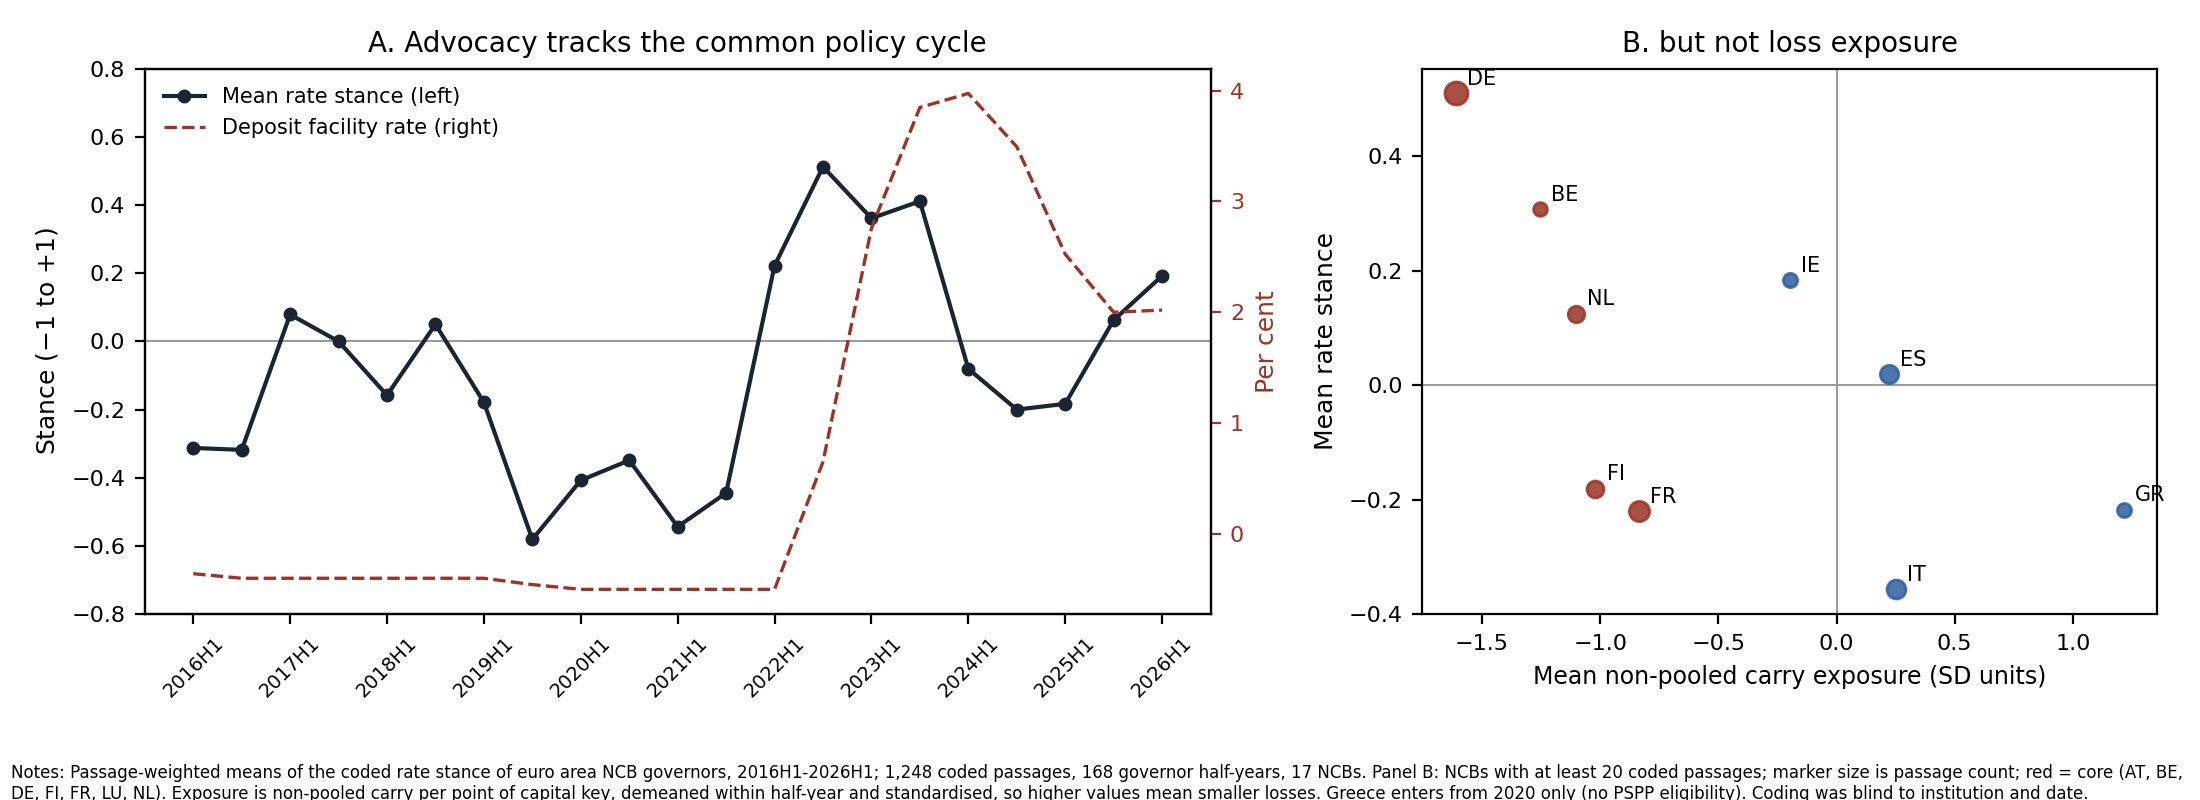
\includegraphics[width=\textwidth]{figures/fig_stance.png}
\caption{Rate advocacy of euro area NCB governors, 2016--2026}\label{fig:stance}
\end{figure}

\begin{figure}[t]\centering

\includegraphics[width=0.78\textwidth]{figures/fig_specifications.png}
\caption{Effect of loss exposure across pre-specified specifications}\label{fig:spec}
\end{figure}

\paragraph{The stance measure.}
Of the 1{,}991 keyword-matched passages, 62.7\% state a view on the policy rate: 389 favour higher rates, 536 are neutral and 323 favour lower rates. Just over a fifth evaluate only past decisions. Aggregating to governor half-years gives 168 cells covering 31 governors and 17 NCBs, built on 1{,}248 coded passages.

Two patterns establish that the measure captures what it is meant to capture, and neither was visible during coding. First, the time profile traces the policy cycle: the passage-weighted mean stance is $-0.54$ in 2021H1, $+0.51$ in 2022H2 at the peak of the tightening, and back to $-0.20$ in 2024H2 once cuts began. Second, the cross-section reproduces the familiar ordering of the Governing Council: Germany $+0.51$, the Netherlands $+0.13$, Spain $+0.02$, Finland $-0.18$, France $-0.22$, Greece $-0.22$, Italy $-0.36$. Core NCBs average $+0.15$, others $-0.11$. Figure~\ref{fig:stance}, panel A, shows the first pattern against the deposit facility rate; panel B plots each NCB's average stance against its average exposure and shows the paper's headline result: the two are unrelated, and the visible ordering of governors runs along the core--periphery line rather than along the loss line.

\paragraph{Exposure does not move advocacy.}
Table~\ref{tab:main} and Figure~\ref{fig:spec} report the pre-specified estimates. The main specification gives
\[
\hat\beta = 0.034 \quad (\text{SE } 0.187,\; t = 0.19,\; p_{\text{perm}} = 0.81),
\]
with a 95\% confidence interval of $[-0.33, 0.40]$. The coefficient has the predicted sign but is an order of magnitude smaller than the spread in average stance across NCBs, and the interval comfortably contains zero.

The raw cross-section runs the other way. Panel B of Figure~\ref{fig:stance} shows that the NCBs with the deepest losses -- Germany, Belgium, the Netherlands, Finland, France -- are on average the more hawkish, because the NCBs that bought low-yielding bonds are the core NCBs whose governors were hawkish throughout. The pooled slope without fixed effects is $-0.165$ and the correlation across NCBs is $-0.59$: read naively, the data would say that larger losses make governors \emph{more} hawkish. This is precisely the confound the fixed effects are there to remove, and once persistent national and personal types are absorbed, nothing is left.

Nothing in the pre-specified robustness set changes this. Replacing governor with NCB fixed effects gives $0.076$; dropping successors appointed after 2022 gives $-0.057$; dropping controls gives $0.016$; using contemporaneous rather than pre-period controls gives $0.010$; excluding purely retrospective passages gives $0.002$; the directional-intensity outcome gives $0.022$. Adding core-by-half-year fixed effects, the check we expected to be most demanding, gives $0.109$ with $p=0.32$. Across the twelve pre-specified constructions of the exposure measure the estimate lies between $0.033$ and $0.046$. Dropping each NCB in turn moves it between $-0.13$ and $+0.11$, with one sign change out of seventeen.

The falsification tests behave as they should under a null. Leads of exposure two half-years ahead give $-0.013$ ($p=0.86$), so there is no pre-trend to explain away. Pre-period debt interacted with the deposit facility rate, entered alongside exposure, is $0.001$ ($t=0.41$): in this design the fiscal channel is as flat as the loss channel.

\begin{figure}[t]\centering
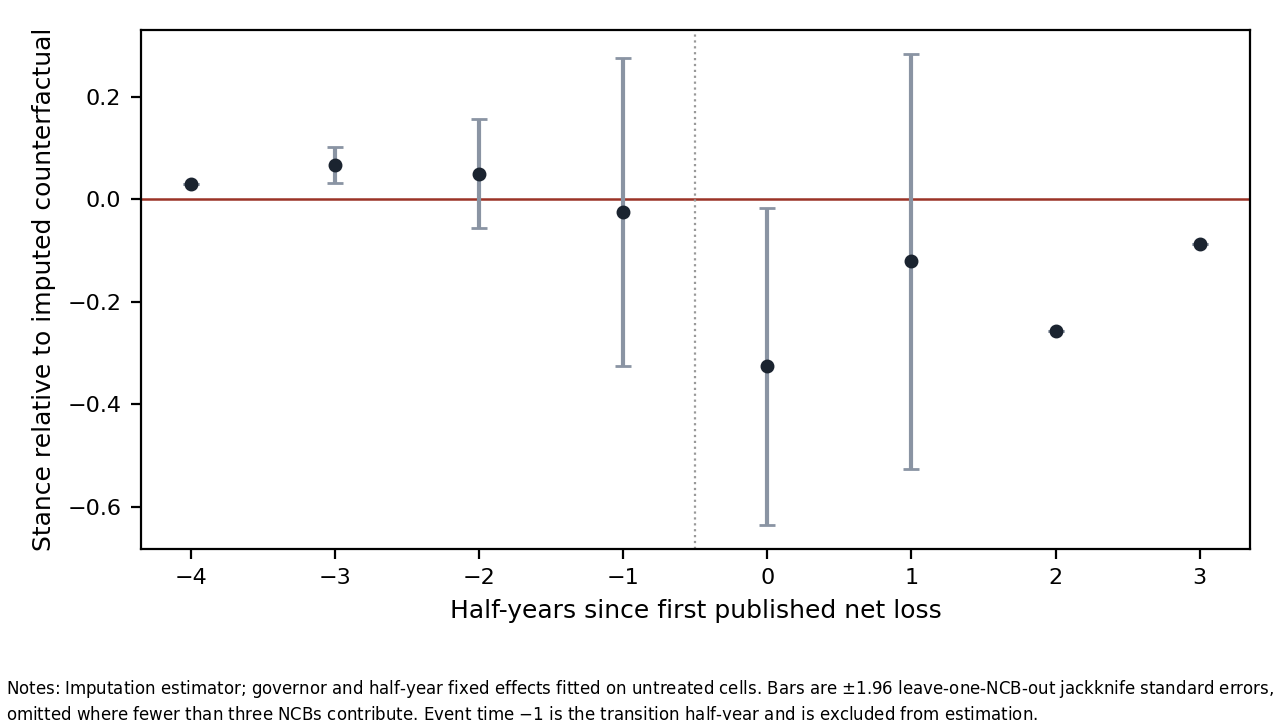
\includegraphics[width=0.72\textwidth]{figures/fig_event.png}
\caption{Advocacy around the first published net loss}\label{fig:event}
\end{figure}

\paragraph{The event design points the right way but proves nothing.}
The imputation estimator around the first published net loss gives an ATT of $-0.163$, in the hypothesised direction, with $p_{\text{perm}}=0.47$; the Callaway--Sant'Anna version gives $-0.143$. Placebo event dates assigned to never-treated NCBs produce an estimate at least this large in absolute value in 64\% of draws. Gross losses fully covered by provisions give $+0.030$, so the difference between a published net loss and a covered loss is $-0.19$ -- the sign predicted by reference dependence, with no precision behind it. Figure~\ref{fig:event} shows the event-time profile. The three pre-treatment coefficients we can estimate with more than two NCBs are $0.07$, $0.05$ and $-0.03$, so there is no pre-trend. The coefficient in the half-year of first treatment is $-0.33$ with a jackknife standard error of $0.16$, and it falls back to $-0.12$ in the following half-year; beyond that only one NCB contributes and we do not interpret the points. Taken at face value the profile looks like a short-lived dovish shift on publication, but the number of treated units is three at impact and four thereafter, the permutation $p$-value is $0.47$, and placebo dates produce something as large in 64\% of draws. We pre-registered this design as underpowered (38 to 55\% against an effect of $0.30$) and report it as suggestive at most. It is, however, the one result in the paper that a follow-up with more treated institutions could turn into something.

\paragraph{How large an effect can we exclude?}
A confidence interval answers this indirectly; an equivalence test answers it directly. Two one-sided tests against a bound of $\pm 0.30$ scale points give a $p$-value of $0.077$: we cannot declare equivalence at that bound. Against $\pm 0.40$ the $p$-value is $0.025$, and the smallest bound we can reject at the 5\% level is $\pm 0.34$. In words: effects larger than about a third of a scale point per standard deviation of exposure are statistically excluded, effects of a quarter of a point are not. Since a third of a scale point is roughly forty per cent of the gap between the average German and the average Italian central banker, the exclusion is economically meaningful without being tight.

\paragraph{Costly actions point the same way, with eight observations.}
Speeches are cheap. Decisions about provisions and distributions are not, and they are taken by the institution rather than by the speaker. We hand-collected eight such actions from seven NCBs. All three actions that strengthen buffers occur after the institution published its first net loss: the National Bank of Belgium changed its reserve and dividend policy in March 2024 and paid no variable dividend for 2024, and the Bundesbank made no transfer for a sixth consecutive year. NCBs that never published a net loss did the opposite, drawing down provisions to absorb gross losses (Spain, Finland, Ireland). This pattern is consistent with institutions responding to published losses, but it is close to mechanical -- an NCB with no published loss cannot take an action ``after'' one -- and with eight events we report it as an illustration rather than as a test.

\paragraph{Where advocacy does come from.}
The null is not the absence of structure. Governor fixed effects alone explain 49\% of the passage-weighted variance of stance, half-year fixed effects alone 42\%, and together 84\%. The residual available to any time-varying national variable is 16\%. Within that residual, exposure retains 9.6\% of its own variance after the fixed effects and the pre-period controls, so the design is not simply collinear: there is variation to use, and it is unrelated to stance.

This is the paper's substantive finding. Stated preferences in the Governing Council decompose almost entirely into a common policy cycle and a stable individual or institutional type. National financial conditions of the speaker's own central bank, including the losses that dominated the public debate from 2023 onward, add nothing measurable on top.

\begin{table}[t]\centering\small
\begin{threeparttable}
\caption{Effect of non-pooled carry exposure on rate advocacy}\label{tab:main}
\begin{tabular}{lccc}
\toprule
Specification & Estimate & $t$ (jackknife) & $p$ (perm.) \\
\midrule
H3 Main (governor and half-year FE, pre-period controls) & 0.034 & 0.18 & 0.81 \\
R1 NCB instead of governor FE & 0.076 & 0.36 & 0.63 \\
R3 Excluding successors appointed after 2022 & $-0.057$ & $-0.35$ & 0.65 \\
R4 No controls & 0.016 & 0.22 & 0.80 \\
R5 Directional-intensity outcome & 0.022 & 0.09 & 0.94 \\
R9 Adding core $\times$ half-year FE & 0.109 & 0.78 & 0.32 \\
R10 Contemporaneous controls & 0.010 & 0.13 & 0.87 \\
R11 Excluding retrospective passages & 0.002 & 0.01 & 0.99 \\
F1 Lead of exposure (two half-years) & $-0.013$ & $-0.15$ & 0.86 \\
F6 Pre-period debt $\times$ DFR, given exposure & 0.001 & 0.41 & 0.51 \\
\midrule
H1 First published net loss (imputation ATT) & $-0.163$ & $-0.66$ & 0.47 \\
R6 First covered gross loss (imputation ATT) & 0.030 & 0.07 & 0.93 \\
R8 Callaway--Sant'Anna, net loss & $-0.143$ & -- & -- \\
\bottomrule
\end{tabular}
\begin{tablenotes}\footnotesize
\item \textit{Notes:} Outcome is the passage-weighted mean rate stance on a $-1$ to $+1$ scale, by governor and half-year, 2016H1 to 2026H1; 168 cells, 31 governors, 17 NCBs, 1{,}248 coded passages. Exposure is the non-pooled carry of own PSPP and PEPP holdings per percentage point of capital key, demeaned across NCBs within each half-year and standardised. Controls are the 2019--2021 averages of the ten-year spread to Germany and of the general government debt ratio, each interacted with the deposit facility rate; national HICP was not available and is a documented deviation. Estimation weights are the number of passages. $t$ uses a leave-one-NCB-out jackknife standard error. $p$ is a permutation $p$-value from 999 permutations of entire exposure paths (H3 and robustness) or of cohort assignments (H1 and R6) across NCBs; its simulated size at the 5\% level is 5.2\%. A null-imposed wild cluster bootstrap-$t$ on 17 NCB clusters gives $p=0.75$ for the main specification. All specifications were fixed before any passage was coded.
\end{tablenotes}
\end{threeparttable}
\end{table}

\section{Why might losses not matter?}\label{sec:discussion}

A null invites the question of what would have had to be true for the answer to be different. We see three explanations, and the data speak to each only partially.

\paragraph{The losses are real but not binding.}
No euro area NCB has been recapitalised, and none has needed to be. Losses are carried forward, provisions absorb part of them, and the sovereign behind each institution is solvent. Under these conditions a governor may regard the published result as an accounting outcome with no consequence for her ability to deliver price stability -- which is exactly what several of them say in the passages we coded, one asking in as many words whether such losses impair the ability of central banks to apply their preferred policy rules and answering that they do not. The prediction that follows is that the effect should appear where the conditions bind: where equity is negative, where statutes require recapitalisation, or where the sovereign is fiscally constrained. Our sample contains one NCB with negative equity and none with a distressed sovereign, so we cannot test this.

\paragraph{The committee aggregates the incentive away.}
Even if individual governors responded, the Governing Council decides collectively and the pooled component of income dominates the non-pooled one. A governor who knows that her vote is one of twenty-one, and that the instrument with the largest effect on her own result -- the remuneration of reserves -- is set for the whole system, has little to gain from bending her stated preference on the policy rate. This is consistent with our finding that the exposure channel and the pre-period debt channel are both flat, since both work through the same collective decision.

\paragraph{Appearing captured is more costly than the loss.}
The passages contain repeated, unprompted denials: that policy is constrained by public finances, that normalisation would be delayed out of concern for treasuries or for losses at individual institutions, that the central bank would accept subordination to fiscal needs. Reputational cost of this kind is a reason to keep stated preferences clean even if the underlying incentive is felt. It has an observable implication we cannot pursue here: the effect should be larger in settings where the incentive can be acted on without being named -- the composition of purchases, the pace of run-off, the design of reserve requirements -- than in public statements about the policy rate.

\paragraph{What would settle it.}
The cleanest test remains the one our corpus could not support. Reducing the remuneration of reserves improves the published result and is neutral for the monetary stance, because the marginal rate remains the deposit facility rate. A policymaker who weights her own result should favour it; one who does not should be indifferent. Euro area governors say too little about this instrument in public for the question to be answered from speeches: 0.38 keyword-matched passages per NCB half-year, most of them descriptive. Answering it requires the voting record, the minutes of the committees that prepare these decisions, or a jurisdiction where the accounting consequences are debated openly.

\section{What we can and cannot conclude}\label{sec:limits}

\paragraph{Power.} The confidence interval on the main estimate runs from $-0.33$ to $+0.40$ scale points. Simulations with the actual distribution of passages put the minimum detectable effect at roughly $0.27$ points per standard deviation at 80\% power. Three benchmarks put that number in context. The full swing of the policy cycle in our measure, from the trough in 2021H1 to the peak in 2022H2, is $1.09$ scale points. The gap between the most hawkish and most dovish NCB average, Germany and Italy, is $0.87$. The standard deviation of average stance across the 31 governors is $0.51$. Our minimum detectable effect is thus about a quarter of the cycle and a third of the core--periphery gap: we can rule out that one standard deviation of loss exposure moves advocacy as much as being a German rather than an Italian central banker, but not that it does a fifth of that. This is a bounded null, not a zero.

\paragraph{Measurement error in the treatment.}
Exposure is constructed, not observed. Classical measurement error in a regressor attenuates the coefficient towards zero, which is exactly the shape of our result, so the null deserves a sharper statement than stability alone provides. Two observations bound the concern without removing it. First, the agreement of the twelve construction variants speaks only to robustness against our own modelling choices, not to the reliability of the common construction; we do not claim otherwise. Second, the only external benchmark -- reported net interest income for four NCBs over two years -- gives a rank correlation of $0.79$ and fails to reproduce the France--Germany ordering. If the reliability ratio of our measure were, say, $0.6$, the attenuation-corrected coefficient at the upper end of the confidence interval would be about $0.67$ rather than $0.40$, and the exclusion region would widen correspondingly. The honest reading is that the equivalence bound we report is a bound on the effect of \emph{our measure} of exposure, and a weaker bound on the effect of true exposure.

\paragraph{Measurement of the outcome.} Passages were coded in a single pass by a language model working from a frozen codebook, with institution, role, country and city masked, and before any link to dates or institutions. There is no independent human validation sample and therefore no human--human or human--model agreement statistic, and no estimate of the recall of the keyword filter. Two consequences follow. Internal consistency is supported -- the coded share, the position distribution and the retrospective share are stable across the whole corpus, and the time and cross-section profiles reproduce facts that were invisible during coding -- but external validity of the coding rule is not established. This is the principal remaining limitation of the measurement design, and we do not treat it as a residual caveat: the substantive contribution is a bounded null, and a bound is only as good as the reliability of the variable it bounds. If the coding is noisier than internal consistency suggests, the effective power is lower than our simulations assume and the exclusion region is correspondingly wider. The full set of coded passages, the frozen codebook and the blind coding interface are in the replication package precisely so that an independent human validation can be run at low cost.

\paragraph{Outcome.} Speeches are not votes. Individual positions in the Governing Council are not published, so we measure what members say rather than how they decide. Our pre-registered second outcome, advocacy on reserve remuneration -- the instrument on which a loss-averse governor has the clearest motive and an inflation-focused one has none -- proved too rare in speeches to be measurable, which is why the sharp sign-pattern test could not be run.

\paragraph{External validity.} Even with a larger sample, the result would speak to a specific configuration: a committee whose members' institutions are not recapitalised automatically but are backed by solvent sovereigns, over one tightening cycle. It says little about a central bank with negative equity and a fiscally constrained government.

\section{Conclusion}

We test, with a design registered in advance, whether the losses that euro area national central banks booked after 2022 changed what their governors advocated on interest rates. They did not, within a band that excludes large effects but not moderate ones. The finding is not that losses are invisible to policymakers: they discuss them, quantify the interest rate risk on their own balance sheets, and defend the decision to accept losses in pursuit of the mandate. The finding is that this discussion leaves no measurable trace in their stated rate preferences, once the common cycle and each speaker's persistent type are taken out -- and that those two things account for 84\% of the variation.

What we still do not know is whether the same holds where it would matter most. The instrument on which loss aversion has its cleanest signature is the remuneration of reserves, and euro area governors say too little about it in public for the question to be settled from speeches. Answering it will require the voting record, or a setting where the accounting consequences of that choice are debated in the open.

\clearpage
\addcontentsline{toc}{section}{References}
\bibliographystyle{plainnat}
\bibliography{refs}

\clearpage
\appendix
\renewcommand{\thesection}{\Alph{section}}
\section{Model: derivations and verification}\label{app:model}

Write the first-order conditions of \eqref{eq:loss} as $F(x;\omega)=\nabla_x L = 0$ with $x=(r,q,a)$, and let $H=\nabla_x F$ be the Hessian. Since $\Pi$ is linear in each instrument, $H$ does not depend on $\omega$ except through the cross-terms, and
\[
H=\begin{pmatrix} \kappa^2+\phi & -\omega D & \kappa\eta+\omega\delta \\[2pt] -\omega D & \chi & 0 \\[2pt] \kappa\eta+\omega\delta & 0 & \eta^2+\zeta \end{pmatrix}.
\]
We consider interior optima at which $H$ is positive definite, which is the second-order condition. Differentiating $F=0$ with respect to $\omega$ and using $\partial F/\partial\omega = -\nabla_x \Pi$ gives the basic comparative-statics relation
\begin{equation}\label{eq:cs}
\frac{\partial x^*}{\partial \omega} \;=\; H^{-1}\,\nabla_x \Pi, \qquad
\nabla_x \Pi = \bigl(-(1-q)D + B - a\delta,\; D r,\; -\delta(r-s)\bigr)'.
\end{equation}

\paragraph{Proof of Proposition~\ref{prop:pnl}.}
The result implied by the advocated mix is $\Pi(x^*(\omega))$. By the envelope-free chain rule and \eqref{eq:cs},
\[
\frac{d\Pi(x^*(\omega))}{d\omega} \;=\; \nabla_x\Pi' \frac{\partial x^*}{\partial\omega} \;=\; \nabla_x\Pi'\,H^{-1}\,\nabla_x\Pi \;\ge\; 0,
\]
with strict inequality whenever $\nabla_x \Pi \neq 0$, because $H$ positive definite implies $H^{-1}$ positive definite. The statement holds for any cost function satisfying the second-order condition and does not depend on which instrument adjusts. \hfill$\square$

\paragraph{Proof of Proposition~\ref{prop:kink}.}
The first-order condition for $q$ is $\chi q - \omega D r = 0$. Evaluated at the prevailing policy rate $r_t$ rather than at the governor's own preferred rate, this gives $q_i^\dagger(r_t) = \omega_i D r_t/\chi$. $D$ is the reserve base per unit of capital key and is pooled, and $r_t$ is common by construction, so at a given date $q^\dagger$ varies across NCBs only through $\omega_i$ or $\chi_i$. Under \eqref{eq:omega}, $\omega_i$ varies either because $\psi_i$ varies or because the loss indicator does. With $\ell=0$ and common $\psi$, $q^\dagger$ is identical across NCBs: linear concern for profit generates no disagreement about the remuneration of reserves. Note that the same statement does not hold for $q_i^*=\omega_i D r_i^*/\chi$ evaluated at each governor's own preferred rate, which inherits variation in $g_i$ through $r_i^*$; the conditioning on $r_t$ is essential. \hfill$\square$

\paragraph{Proof of Proposition~\ref{prop:rate}.}
Write $A=\kappa^2+\phi$, $C=\kappa\eta+\omega\delta$, $E=\eta^2+\zeta$, so that
\[
H=\begin{pmatrix} A & -\omega D & C \\ -\omega D & \chi & 0 \\ C & 0 & E\end{pmatrix},\qquad
\nabla_x\Pi=\begin{pmatrix} -\Lambda \\ D r \\ -\delta(r-s)\end{pmatrix},\qquad \Lambda \equiv (1-q)D - B + a\delta .
\]
The first row of $H^{-1}$ is $\bigl(\chi E,\; \omega D E,\; -\chi C\bigr)/\det H$, and $\det H>0$ under the second-order condition. Hence
\[
\frac{\partial r^*}{\partial\omega} \;=\; \frac{\chi E\,(-\Lambda) + \omega D E\,(D r) + (-\chi C)\bigl(-\delta(r-s)\bigr)}{\det H}
\;=\; \frac{E\bigl[\omega D^2 r - \chi\Lambda\bigr] + \chi\,\delta(r-s)\,(\omega\delta+\kappa\eta)}{\det H}.
\]
This is negative if and only if $\chi E\Lambda > \omega D^2 E r + \chi\delta(r-s)(\omega\delta+\kappa\eta)$, which on dividing by $\chi E$ and substituting $q^* = \omega D r/\chi$ is exactly condition~\eqref{eq:cond}. Setting $\delta=0$ leaves $\chi E\Lambda > \chi E q^* D$, that is $(1-q^*)D-B > q^*D$, or $D(1-2q^*)>B$. \hfill$\square$

We verify the algebra numerically: across 266 admissible parameter draws the sign of $\partial r^*/\partial\omega$ agrees with condition~\eqref{eq:cond} in every draw, and the closed-form expression above reproduces the numerically differentiated derivative to machine precision. The earlier version of this appendix reported that the sign could only be signed under additional sufficient conditions; the equivalence above supersedes that statement.

\paragraph{Predictions that fail.}
The same procedure rejects two predictions. First, $\partial a^*/\partial\omega<0$ holds in only 65 of the 266 admissible draws: when $\delta(r-s)$ is small relative to $\Lambda$, a governor who lowers the costly rate substitutes into sales, and the second effect dominates. Second, $\partial a^*/\partial\delta<0$ holds in 251 of 266 draws, because duration enters both the loss per sale and the rate exposure. Neither is used in the empirical work. We report them because the numerical check is the reason the empirical design does not contain a sign-pattern test on asset sales.

\paragraph{Stance neutrality at $\omega=0$.}
Setting $\omega=0$ in the first-order conditions gives $q^*=0$ and, symbolically,
\[
\frac{\partial r^*}{\partial g}\Big|_{\omega=0}=\frac{\kappa\zeta}{\eta^2\phi+\kappa^2\zeta+\phi\zeta}>0,\qquad
\frac{\partial a^*}{\partial g}\Big|_{\omega=0}=\frac{\eta\phi}{\eta^2\phi+\kappa^2\zeta+\phi\zeta}>0,\qquad
\frac{\partial q^*}{\partial g}\Big|_{\omega=0}=0 .
\]
A governor who cares only about stabilisation raises the rate and sells more when she perceives more inflation pressure, and is indifferent about the remuneration of reserves. This is the formal content of the claim that advocacy on reserve remuneration would have separated loss aversion from preference shifters.

\section{Data construction}\label{app:data}
\paragraph{Speaker affiliation.} BIS descriptions follow the pattern ``Type by Title Name, Role of Institution, at Venue, Place, Date''. We remove the speaker name, cut the string at the first venue marker and match institution aliases only in the remaining affiliation segment. Roles containing deputy, vice, member, director, chief, adviser or head of are classified as non-heads. Twelve unit tests use real descriptions, including joint speeches and speeches hosted by another central bank.
\paragraph{Masking.} Before coding, speaker names (all BIS authors), institution names and aliases, role phrases, country names, demonyms and 21 capitals and major cities are replaced by placeholders. An automated scan finds residual country cues in 3 of 400 validation passages.
\paragraph{Published results.} For each NCB and financial year we record the pre-provision result, provisions released, net result, loss carried forward, transfer to the state, publication date and one source (annual accounts, press releases, audit reports or press coverage of the accounts). Values derived rather than read are flagged in the file.
\paragraph{Exposure.} Holdings are cumulative monthly net purchases by jurisdiction from the ECB PSPP and PEPP histories; our parsed values reproduce the ECB's published tables. The NCB-own share of jurisdiction holdings is 8/9. Purchase yields are national ten-year yields shifted to the portfolio's weighted average maturity using the slope of the AAA euro area curve. The reference rate is the monthly average MRO rate until December 2024 and the deposit facility rate from January 2025. Carry is divided by the Eurosystem capital key (2024 key before 2024, 2026 key from 2026). Table~\ref{tab:grid} reports the pre-specified construction variants.
\paragraph{Debt ratios.} General government gross debt in percent of GDP, 2019 to 2021, from Eurostat news release 118/2022 (second EDP notification 2022).

\begin{table}[h]\centering\small
\begin{threeparttable}
\caption{Exposure construction variants}\label{tab:grid}
\begin{tabular}{lcc}
\toprule
Variant & Rank corr.\ & Corr.\ with \\
(redemptions, PEPP share, maturity) & with NII & baseline \\
\midrule
net flow, 8/9, 1.0 (baseline) & 0.79 & 1.00 \\
net flow, 8/9, 0.75 & 0.81 & 1.00 \\
net flow, 8/9, 1.5 & 0.79 & 1.00 \\
net flow, 1.0, 0.75 / 1.0 / 1.5 & 0.79 & 1.00 \\
ladder, 8/9 or 1.0, 0.75 & 0.74 & 0.99 \\
ladder, 8/9 or 1.0, 1.0 & 0.76 & 0.99 \\
ladder, 8/9 or 1.0, 1.5 & 0.79 & 0.98 \\
\bottomrule
\end{tabular}
\begin{tablenotes}\footnotesize
\item \textit{Notes:} Rank correlation between annual carry per key point and net interest income after reallocation per key point for Germany, France, Italy and Spain in 2023 and 2024 (eight observations; source \citealp{arrata2026}). Correlation with the baseline uses demeaned half-year carry per key point from 2022H1 onwards. The PEPP share does not affect demeaned carry per key point when the ladder method is used, and changes it only marginally under net flows.
\end{tablenotes}
\end{threeparttable}
\end{table}

\section{Codebook for rate stance}\label{app:codebook}
\textit{Topic.} The passage states or reports a view on the direction, level or pace of policy rates or on the overall monetary policy stance. Not on topic: inflation or growth forecasts without reference to policy, statements only on the balance sheet or asset purchases, regulation and other topics.
\textit{Position.} $-1$: favours lower rates, cuts, earlier or larger cuts, slower or smaller hikes, or warns against over-tightening. $+1$: favours higher rates, hikes, faster or larger tightening, or warns against easing too early. $0$: neutral, purely reporting, data-dependent without direction, or balanced.
\textit{Rules.} Only the speaker's own view counts. Defending past hikes is $+1$ and defending past cuts $-1$. ``We should not cut yet'' is $+1$. ``Rates stay; decisions depend on data'' without contrast is $0$.
\textit{Retrospective.} The passage only evaluates past decisions and says nothing about the future course.

\section{Simulation evidence on inference and power}\label{app:sim}
All simulations use the actual number of keyword-matched passages per NCB and half-year and the observed exposure paths or cohorts. Assumptions: passage noise standard deviation 0.7 on the $-1$ to $+1$ scale, governor-half-year shock 0.2, 60\% of keyword-matched passages on topic.

\begin{table}[h]\centering\small
\begin{threeparttable}
\caption{Size and power}\label{tab:sim}
\begin{tabular}{llccccc}
\toprule
Design & Inference & Size & \multicolumn{4}{c}{Power at effect size} \\
 & & & 0.15 & 0.20 & 0.25 & 0.30 \\
\midrule
Exposure, no controls & RI, raw coefficient & 0.17 & & & & \\
Exposure, no controls & RI, CR0 $t$ & 0.06 & 0.66 & 0.83 & & \\
Exposure, controls & RI, CR0 $t$ & 0.09 & & 0.81 & 0.90 & \\
Exposure, controls & RI, jackknife $t$ & 0.05 & 0.38 & 0.55 & 0.74 & 0.88 \\
Published loss (H1) & RI, ATT & 0.06 & 0.15 & 0.24 & & 0.38 \\
\bottomrule
\end{tabular}
\begin{tablenotes}\footnotesize
\item \textit{Notes:} Exposure effects in scale points per standard deviation of exposure; published-loss effects in scale points. Size is the rejection rate at the 5\% level under a true null (400 to 600 replications). Rows with size above 0.05 are shown to document why they were not adopted. Power for rows with invalid size is not interpretable.
\end{tablenotes}
\end{threeparttable}
\end{table}



\begin{table}[t]\centering\small
\begin{threeparttable}
\caption{All exposure constructions and leave-one-out estimates}\label{tab:all}
\begin{tabular}{lcc@{\hskip 2em}lcc}
\toprule
\multicolumn{3}{l}{\textit{Panel A: exposure constructions}} & \multicolumn{3}{l}{\textit{Panel B: dropping one NCB}} \\
Construction & $\hat\beta$ & $t$ & Dropped & $\hat\beta$ & $t$ \\
\midrule
Net flow, 8/9, 0.75 & 0.036 & 0.18 & Italy & $-0.130$ & $-0.50$ \\
Net flow, 8/9, 1.0 (baseline) & 0.034 & 0.18 & Malta & 0.002 & 0.01 \\
Net flow, 8/9, 1.5 & 0.033 & 0.19 & Estonia & 0.009 & 0.04 \\
Net flow, 1.0, 0.75 & 0.036 & 0.19 & Ireland & 0.026 & 0.13 \\
Net flow, 1.0, 1.0 & 0.035 & 0.19 & Cyprus & 0.034 & 0.18 \\
Net flow, 1.0, 1.5 & 0.034 & 0.19 & Austria & 0.034 & 0.18 \\
Ladder, 8/9, 0.75 & 0.045 & 0.27 & Lithuania & 0.034 & 0.18 \\
Ladder, 8/9, 1.0 & 0.042 & 0.26 & Slovakia & 0.034 & 0.19 \\
Ladder, 8/9, 1.5 & 0.040 & 0.26 & Slovenia & 0.035 & 0.19 \\
Ladder, 1.0, 0.75 & 0.046 & 0.28 & Portugal & 0.036 & 0.19 \\
Ladder, 1.0, 1.0 & 0.044 & 0.27 & Belgium & 0.037 & 0.20 \\
Ladder, 1.0, 1.5 & 0.041 & 0.27 & Finland & 0.042 & 0.21 \\
 & & & France & 0.048 & 0.24 \\
 & & & Germany & 0.049 & 0.22 \\
 & & & Netherlands & 0.050 & 0.32 \\
 & & & Spain & 0.085 & 0.78 \\
 & & & Greece & 0.106 & 0.67 \\
\bottomrule
\end{tabular}
\begin{tablenotes}\footnotesize
\item \textit{Notes:} Panel A varies the three pre-specified construction choices: redemption treatment (net flow or uniform maturity ladder), the NCB share of PEPP holdings (8/9 or 1), and purchase maturity as a multiple of the weighted average maturity (0.75, 1.0 or 1.5). Panel B re-estimates the main specification omitting one NCB at a time. All estimates use governor and half-year fixed effects, pre-period controls and passage weights; $t$ uses leave-one-NCB-out jackknife standard errors. The largest movement, dropping Italy, reflects that NCB's share of the identifying variation (Section~\ref{sec:strategy}).
\end{tablenotes}
\end{threeparttable}
\end{table}

\section{Pre-registration and deviations}\label{app:prereg}
The analysis plan (v2) and four amendments (v2.1 to v2.4) were frozen with SHA-256 hashes before any rate-stance passage was read. The sequence, with the data visible at each point, was:
\begin{enumerate}\itemsep2pt
\item[v2] Design fixed: rate stance as the outcome, exposure and published net loss as the two treatments, falsification tests, inference. Triggered by a pre-specified count rule showing that advocacy on reserve remuneration appears in only 0.38 passages per NCB half-year, below the registered threshold of one, so the original outcome was abandoned before any position was coded.
\item[v2.1] Ex-ante power with the realised passage counts: the event design has a minimum detectable effect above 0.4 scale points, the exposure design 0.27. The exposure design becomes primary, the event design secondary and disclosed as underpowered.
\item[v2.2] Controls changed from contemporaneous spread and debt to their 2019--2021 averages interacted with the policy rate, because the contemporaneous versions respond to the same policy decisions. A collinearity rule was registered for the case that the debt control absorbed the exposure variation; it was not triggered (the control leaves 99\% of the post-fixed-effects exposure variance intact).
\item[v2.3] Inference changed from cluster-robust to leave-one-NCB-out jackknife studentisation, after simulations showed rejection rates of 17\% (raw coefficient) and 9\% (cluster-robust $t$) under a true null, against 5.2\% for the jackknife statistic.
\item[v2.4] Leave-one-NCB-out estimates added as a required exhibit, after a diagnostic showed that Greece and Italy alone account for two thirds and two fifths of the identifying variation.
\end{enumerate}

Deviations from the plan, all logged with dates: national HICP could not be retrieved before estimation and is omitted from the controls, and we were subsequently unable to assemble the full country panel from accessible sources, so the post-registered robustness check with inflation remains outstanding; the validation sample was not coded by humans, so the registered agreement gate could not be applied and the heterogeneity tests conditional on governor attributes were skipped for insufficient coverage (23\% and 36\% of passages); the Executive Board placebo requires a further 2{,}451 passages that have not been coded. Two model predictions were dropped after the propositions failed numerical verification, before any data work (Appendix~\ref{app:model}).

\section{Additional results}\label{app:extra}
\paragraph{Variance decomposition.} On the 168 governor half-years, weighting by passages, half-year fixed effects alone explain 41.9\% of the variance of the stance measure, governor fixed effects alone 48.6\%, and the two together 83.8\%.
\paragraph{Exposure variants.} Across the twelve pre-specified constructions (net-flow versus ladder redemptions, NCB share of PEPP holdings of 8/9 versus 1, purchase maturity of 0.75, 1 and 1.5 times the weighted average maturity) the estimate ranges from 0.033 to 0.046.
\paragraph{Leave one out.} Dropping each of the seventeen NCBs in turn gives estimates between $-0.13$ and $+0.11$; the sign changes once. Under the rule registered in v2.4 this would have required us to report the result as carried by individual central banks had the estimate been significant; with a null it simply confirms that no single NCB is driving the zero.
\paragraph{Placebo event dates.} Assigning the observed treatment cohorts at random to never-treated NCBs produces an event-study estimate at least as large in absolute value as the true one in 64\% of 495 draws.

\section{Replication package}\label{app:repl}
The package contains the code, hand-collected data, derived inputs, the frozen pre-analysis plan and amendments, the classification prompts and all raw model responses. A master sequence runs the parser and keyword filter, builds exposure and treatment data, evaluates the collinearity rule, runs the validation analysis and, once classification results are hash-frozen, the estimation. The BIS speeches extract and ECB statistics are public; their terms of use are documented in the README.

\end{document}
